\section{Aufbau der Lehrveranstaltung}

In dieser Lehrveranstaltung soll theoretisches Wissen eng mit praktischer Umsetzung verbunden werden. D.h. zu allen Kapiteln der LV werden praktische Aufgaben, am Beispiel einer Lernfabrik, der sogenannten "Teaching Factory" aus Abbildung \ref{fig:virtuelleFabrik}, gestellt. Die Leistungserbringung wird durch die Umsetzung der Aufgaben und deren Dokumentation erbracht. Dabei wird zwischen Basisaufgaben, diese müssen umgesetzt werden, und optionale Aufgaben, zum erreichen einer besseren Note, unterschieden, mehr dazu im Kapitel \ref{sec:Prüfungsmodalitaet}. Zur Umsetzung der Aufgaben ist TwinCAT 3 von Beckhoff, ein Entwicklungsprogramm für die Beckhoff Soft-SPS, die benötigte Sofware, siehe Kapitel \ref{sec:Software}. Ein Windows Betriebssystem ist für die Installation notwendig. 

Die genaue Aufgabenstellung der Basis- und optionalen Aufgaben finden Sie am Ende jedes Kapitels mit dem Titel Basisaufgabe oder Optionale Aufgabe. 



In der Vorlesung zur Automatisierungstechnik werden grundlegende Konzepte und Technologien behandelt, beginnend mit den Grundlagen der Automatisierungstechnik mit Speicherprogrammierbaren Steuerungen (SPS), in Kapitel \ref{cpt:Grundlagen}. Hierbei werden den Studierenden die Prinzipien und Arbeitsweisen von SPS vermittelt, einschließlich der Funktionsweise, Programmierung und grundlegenden Schaltungs- und Steuerungstechniken.

Ein weiterer wichtiger Aspekt ist die Steuerung von Motoren, in Kapitel \ref{cpt:Motorsteuerung}, bei der die Studierenden Einblicke in elektrische Antriebssysteme erhalten. Die Steuerung von Gleichstrom- und Schrittmotoren sowie die Anwendung von Regelungstechniken für eine präzise Motorsteuerung stehen im Fokus.

Die Entwicklung von Steuerungsprogrammen aus Kapitel \ref{cpt:Steuerungsprogramme} deckt verschiedene Programmiermethoden und -sprachen für Automatisierungssysteme ab. Die Studierenden erlernen den Entwurf und die Implementierung von Steuerungsprogrammen, einschließlich Simulation und Test von Steuerungslogik.

Im Kapitel \ref{cpt:MessSteuerkette} der Mess- und Steuerkette liegt der Fokus auf dem Aufbau und der Funktionsweise von Mess- und Regelungssystemen. Dabei werden Sensorik und Aktorik in der Automatisierungstechnik behandelt, ebenso wie Aspekte der Kalibrierung und Messdatenerfassung.

Sicherheitstechnik ist ein weiterer Schwerpunkt, siehe Kapitel \ref{cpt:Sicherheitstechnik}, der Sicherheitsnormen, Risikobewertung, und Gefahrenanalyse in der Automatisierungstechnik umfasst. Die Studierenden lernen die Implementierung von Sicherheitsfunktionen sowie den Einsatz von Sicherheitskomponenten und -systemen.

Das Kapitel \ref{cpt:Fehlerbehandlung} der Fehlerbehandlung befasst sich mit Diagnose und Fehleranalyse in Automatisierungssystemen. Es werden Redundanzkonzepte für erhöhte Zuverlässigkeit sowie Methoden zur Fehlerbehebung und Wartung von Automatisierungssystemen behandelt.

Im Kapitel \ref{cpt:Kommunikation} der serielle Kommunikation werden verschiedenen Kommunikationsprotokollen in der Automatisierungstechnik, einschließlich Feldbussen und industriellen Netzwerken, besprochen. Die Studierenden erhalten Einblicke in Datenübertragung und -sicherheit.

Abschließend behandelt das Kapitel \ref{cpt:HMI} Human-Machine Interface (HMI) die Gestaltung von Benutzerschnittstellen, die Visualisierung von Prozessdaten und die Interaktion zwischen Mensch und Maschine. HMI-Entwicklungstools und -Methoden runden die Vorlesung ab. Praxisnahe Beispiele, Fallstudien und praktische Übungen werden integriert, um den Studierenden eine umfassende Kenntnis der Automatisierungstechnik zu vermitteln, insbesondere im Hinblick auf deren Anwendung in verschiedenen industriellen Kontexten.




Die Prüfungsleistung wird durch die Umsetzung von Übungen auf der Teaching Factory erfüllt. Es ist eine Gruppengröße von drei Personen einzuhalten. Bei den Übungen gibt es eine Aufteilung zwischen fünf "Pflichtübungen" und 6 optionalen Übungen. Mit den Pflichtübungen können bei korrekter Durchführung und passender Dokumentation 80 Punkte erreicht werden. Diese Übungen sind auf der virtuellen Fabrik umsetzbar, nur die letzte Übung zum Thema Fehlerdetektion kann auf der realen Anlage getestet werden. Die optionalen Übungen sind hauptsächlich auf der realen Anlage durchzuführen. Auf Grund der begrenzten Hardware wird hierzu ein Zeitplan in der Vorlesung, gemeinsam mit den Studenten, erarbeitet. Die genaue Punkteverteilung ist in Tabelle \ref{tab:Pruefungsmodalitaet} aufgelistet. 




\subsection{Benötigte Software} \label{sec:Software}

TwinCAT 3 von Beckhoff, ist eine Entwicklungsumgebung für TwinCAT Runtime Soft-SPS, eingebettet in Microsoft Visual Studio. Bei nicht vorhandener Visual Studio Installation wird eine Shell Umgebung beim Download automatisch installiert. Der Download Link ist mit angelegten Account auf der Beckhoff Homepage verfügbar. 

Um eine virtuelle Inbetriebnahme durchführen zu können und somit die benötigte Zeit an der, begrenzt zur Verfügung stehenden, Hardware zu minimieren, ist eine virtuelle Fabrik, zu sehen in Abbildung \ref{fig:virtuelleFabrik} zur Verfügung gestellt. Diese kann von Sakai heruntergeladen werden.  

\begin{figure}[H]
	\begin{center}
		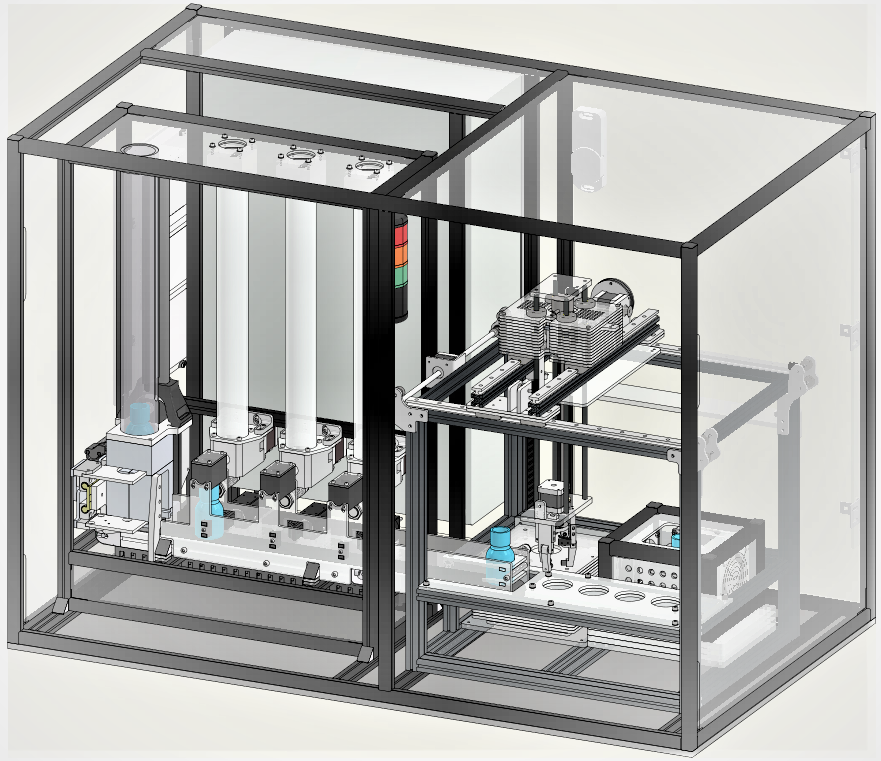
\includegraphics[width=0.8\textwidth]{images/Teaching_Factory_2_3d_GesamteAnlage.png}
		\caption{Virtuelle Fabrik, die sogenannte Teaching Factory.}
		\label{fig:virtuelleFabrik}
	\end{center}	
\end{figure}


\subsubsection{Installationsleitfaden}

Der Download von TwinCAT 3 XAE kann unter dem Link \url{https://www.beckhoff.com/de-at/produkte/automation/twincat/texxxx-twincat-3-engineering/te1000.html?} vorgenommen werden oder durch manuelle Navigation auf der Homepage von Beckhoff unter folgendem Pfad:
www.Beckhoff.com - Account erstellen und anmelden - Produkte/Automation-Produktübersicht/TwinCAT/TExxxx | TwinCAT 3 Engineering/TE1000 | TwinCAT 3 Engineering - Mehr erfahren/Dokumentation und Downloads/Software und Tools/TwinCAT 3 Download | eXtended Automation Engineering (XAE).  
In diesem Bereich die EXE Datei herunterladen und installieren. 

Der Leitfaden zur Installation befindet sich im Beckhoff-Infosys unter dem Link \url{https://infosys.beckhoff.com/index.htm}. Navigieren Sie zum Pfad TwinCAT 3/Installation/Installation bis TwinCAT 3.1 Build 4024/Installation von TwinCAT 3 Engineering und Runtime/ TwinCAT 3 Engineering und Runtime installieren. Befolgen Sie bei der Installation die Angaben der Seite. 

\subsubsection{Setup \& Troubleshooting}

Nach der Installation müssen sowohl für Windows 10 als auch Windows 11 Betriebssysteme weiter Setup Einstellungen getätigt werden. Dazu wird ein Batch-File ausgeführt und anschließend der PC Neu gestartet. Das Batch-File befindet sich im nativen Installationsordner, welcher bei einer Standardinstallation unter folgendem Pfad aufzufinden ist: C:\textbackslash\,TwinCAT\textbackslash3.1\textbackslash\,System\textbackslash\,win8settick.bat. Dieses File als Administrator ausführen und den PC Neustarten.

\textbf{Troubleshooting Windows 10}

Kann nach Ausführung des Batch-Files ein Programm in der Laufzeit von Beckhoff "TwinCAT Runtime" nicht ausgeführt werden, durch den Fehler "Vitualisierungsfunktion Intel VT-x deaktiviert", ist die Ursache demnach, dass die Virtualisierungsfunktion Intel VT-x (bzw. bei älteren PC's nur VT) deaktiviert ist und aktiviert werden muss. Dies kann im Bios des PC's eingestellt werden. 

Suchen Sie im Internet nach ihrem PC Hersteller und welche Tasten bei Booten gedrückt werden müssen um das Bios zu öffnen. Im Anschluss navigieren Sie in den Reiter Sicherheit/Systemsicherheit oder einem ähnlichen Menüpunkt, wie Erweiterte BIOS-Funktionen oder Erweiterte Intel Virtualisierungstechnologie. Aktivieren Sie Virtual Technologie(VTx) und/oder Virtual Technology Directed I/O (VTd). 
Speichern Sie die Änderungen, beenden Sie das BIOS und starten Sie ihren Computer neu. 

\textbf{Troubleshooting Windows 11}

Kann nach Ausführung des Batch-Files ein Programm in der Laufzeit von Beckhoff "TwinCAT Runtime" nicht ausgeführt werden, durch Fehler, wie "start of real-time avoided by Hyper V", "RTIME: Incompatible software detected", können diese Fehler durch vielseitige Ursachen ausgelöst werden. Bitte gehen Sie die folgenden Schritte durch und testen Sie die Runtime-Funktionalität nach jedem Schritt. 
  
  \begin{itemize}
  	\item Deaktivieren von Hyper-V, Virtual Machine Platform und Windows Hypervisor Platform, siehe Anhang \ref{fig:TSHyperV1}
  	\item Deaktivieren von "Core Isolation/Memory Integrity", siehe Anhang \ref{fig:TSHyperV2}
  	\item Zuweisung eines isolierten Kerns, siehe Anhang \ref{fig:TSHyperV3} und Infosys unter Industrie-PC/Betriebssysteme und Tools/TwinCAT BSD/TwinCAT 3/Isolierte Kerne zuweisen
  	\item Deaktivieren der "Virtualization based security", siehe Anhang \ref{fig:TSHyperV4} bzw. \ref{fig:TSHyperV5}
  	\item Ausführen von "bcdedit /set hypervisorlaunchtype off" als Admin
  \end{itemize}


 
\newpage
